\documentclass[english]{article}
\usepackage[T1]{fontenc}
\usepackage[latin9]{inputenc}
\usepackage{babel}
\usepackage{graphicx}
\usepackage{subfigure}
\usepackage{float}
\setlength{\parindent}{0pt}
\usepackage{amsmath}


\begin{document}

\title{Lab 1: Polarization Imaging\\ -------------------------------- \\ \Large Sensors and Digitization}
\author{ \ Armine Vardazaryan, Songyou Peng \\ arminevardazaryan@gmail.com, psy920710@gmail.com}
\date{18th November 2015}

\maketitle

\section{Introduction}

\section{Simplified polarization imaging}
Firstly, in order to answer the fifth question in the "\textbf{Getting started}" part, we rotate the polarizer from 0\textdegree to 90\textdegree. 
The result can be seen in the Figure \ref{fig:one}. Please notice the cellphone screen in the pictures. When the angle of polarizer is 0\textdegree, the screen has a really high intensity, with the 90\textdegree one an extremely low intensity. Due to that, we are able to say that this cellphone are polarized in the direction of 0\textdegree.\\

\begin{figure}[H]
	\centering
	\subfigure[0\textdegree]{\label{fig:onea}
	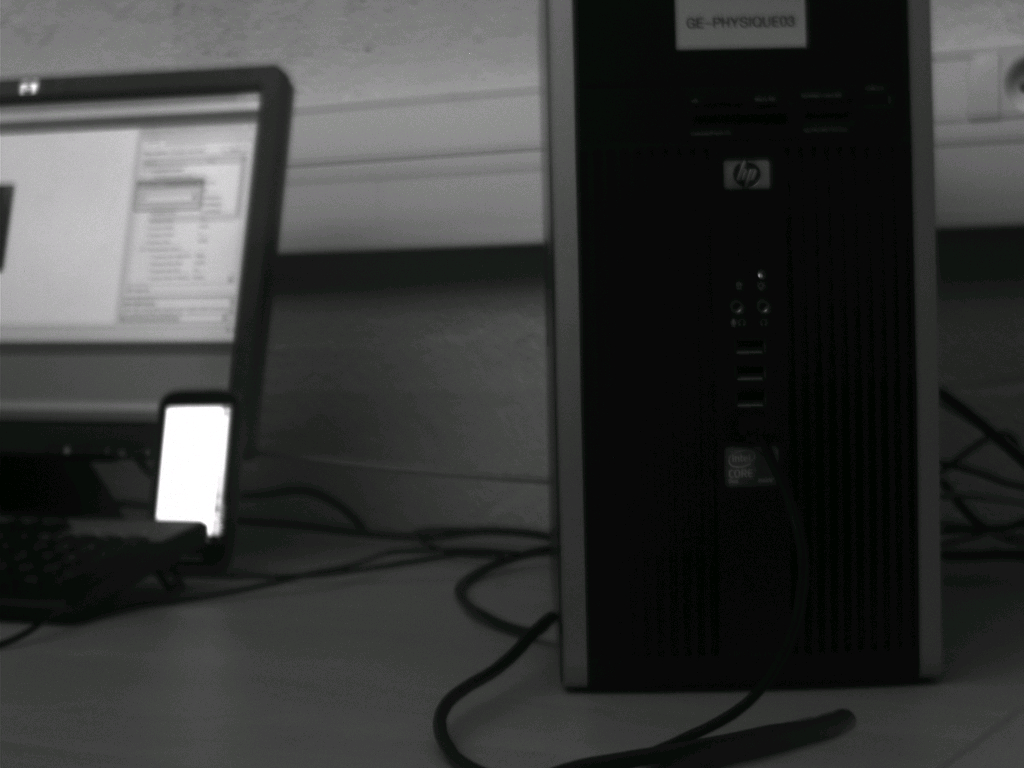
\includegraphics[width=0.3\linewidth]{Pictures/wolff/0.jpg}
	}
	\subfigure[45\textdegree]{\label{fig:oneb}
	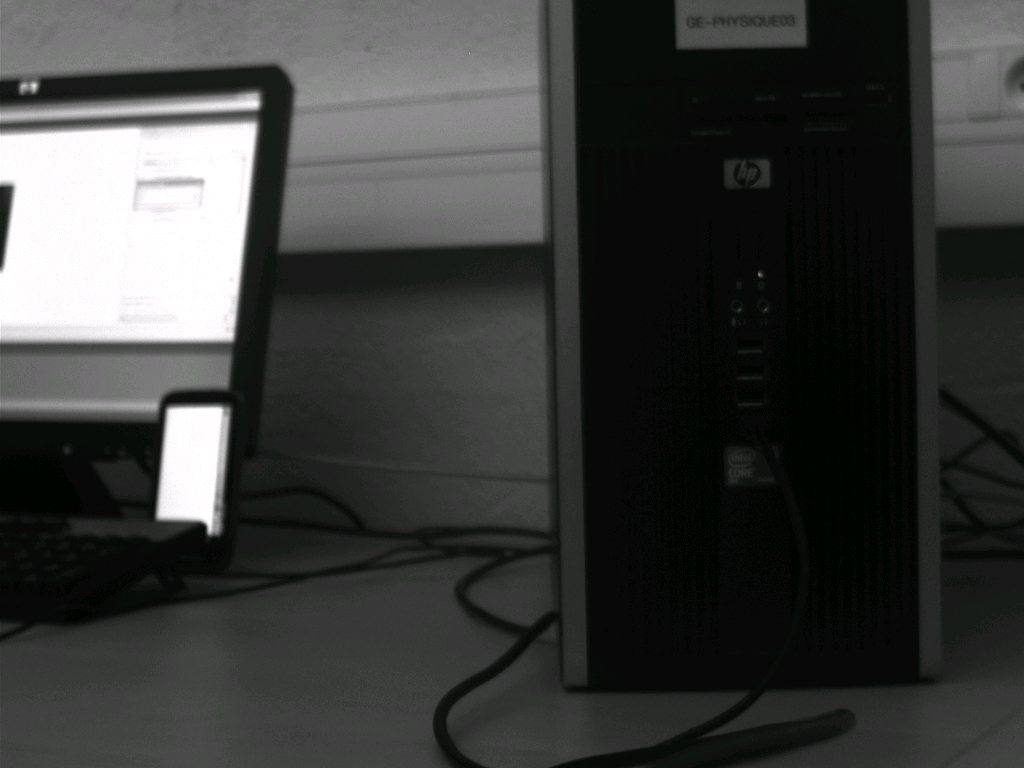
\includegraphics[width=0.3\linewidth]{Pictures/wolff/45.jpg}
	}
	\subfigure[90\textdegree]{\label{fig:onethree}
	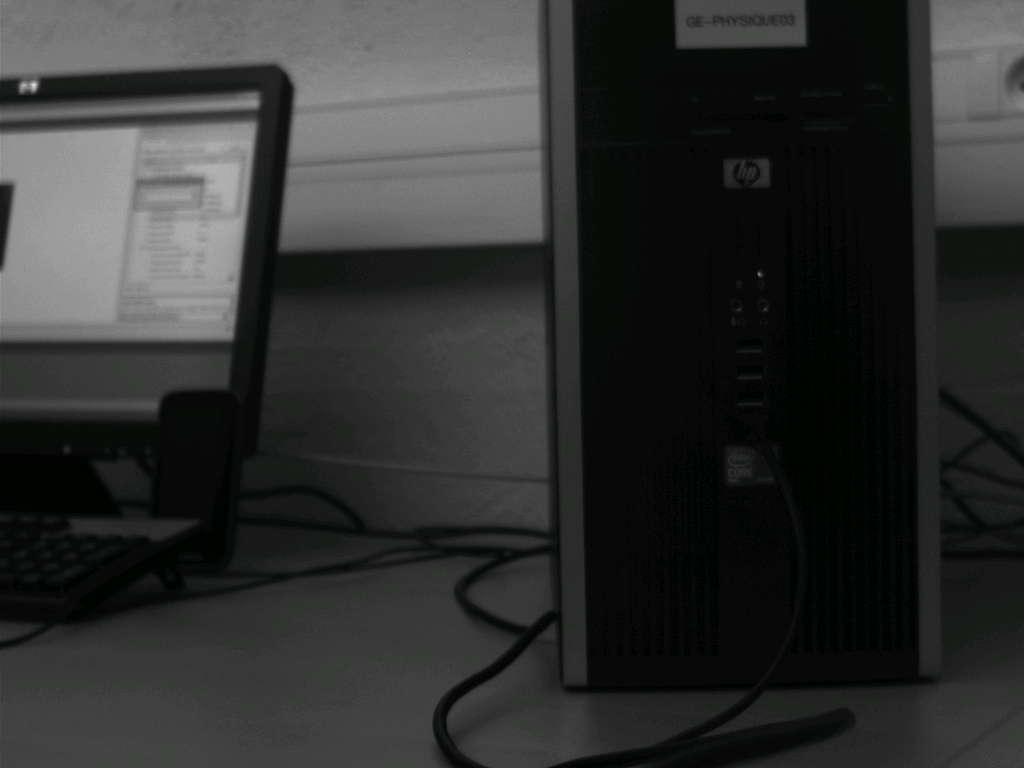
\includegraphics[width=0.3\linewidth]{Pictures/wolff/90.jpg}
	}
	\caption{Pictures in different angles of polarizer}
	\label{fig:one}
\end{figure}

\subsection{Wolff's method}
Before taking any pictures, we set the autoexposure and gain of the camera to be manual because we want to keep everything of camera the same, so that we can eliminate any effect from camera itself.\\
\\
After taking pictures with the polarizer orientation: 0\textdegree, 45\textdegree, 90\textdegree, we first compute the total light intensity $I$, angle of polarization $\varphi$, and degree of polarization $\rho$ respectively. :

\begin{align*} 
	I &= I_{0} + I_{90}\\
	\varphi &= \frac{I - 2I_{45}} {I - 2I_{90}}\\
	\rho &= \frac{\sqrt{(I-2I_{45})^{2} + (I-2I_{90})^{2}}}{I}
\end{align*}

These parameter images are shown respectively in the Figure \ref{fig:two}. We notice in the Figure \ref{fig:twob}, the screens of both computer monitor and smartphone are very dark. In contrast, other region are full of random noise. This is due to the fact the screens are polarized and the light coming out of the screen has only one direction, while other regions in the picture are unporlarized, so the angle of light are in every direction. So this picture reflects the angle of light. \\
\\
In the Figure \ref{fig:twoc}, we find out that the two screens are rather bright while most of other areas are kind of dark. After analysing the reason, we find out this image is about the degree of polarization, which means the brighter a certain area, the higher degree of polarization. That is to say, the screen of computer and smartphone are almost linear polarized, but other objects in the picture are not polarized. So the value in the regions of the screen is  high.

\begin{figure}[H]
	\centering
	\subfigure[Intensity]{\label{fig:twoa}
	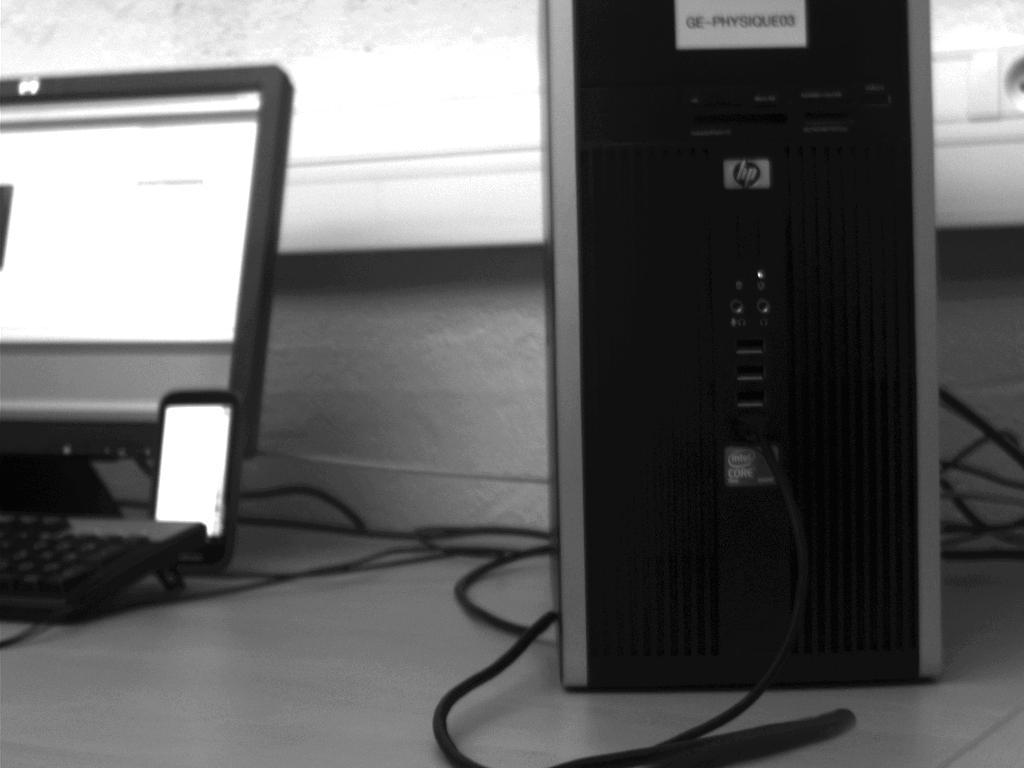
\includegraphics[width=0.3\linewidth]{Pictures/wolff/I.jpg}
	}
	\subfigure[Angle of Polarization $\varphi$]{\label{fig:twob}
	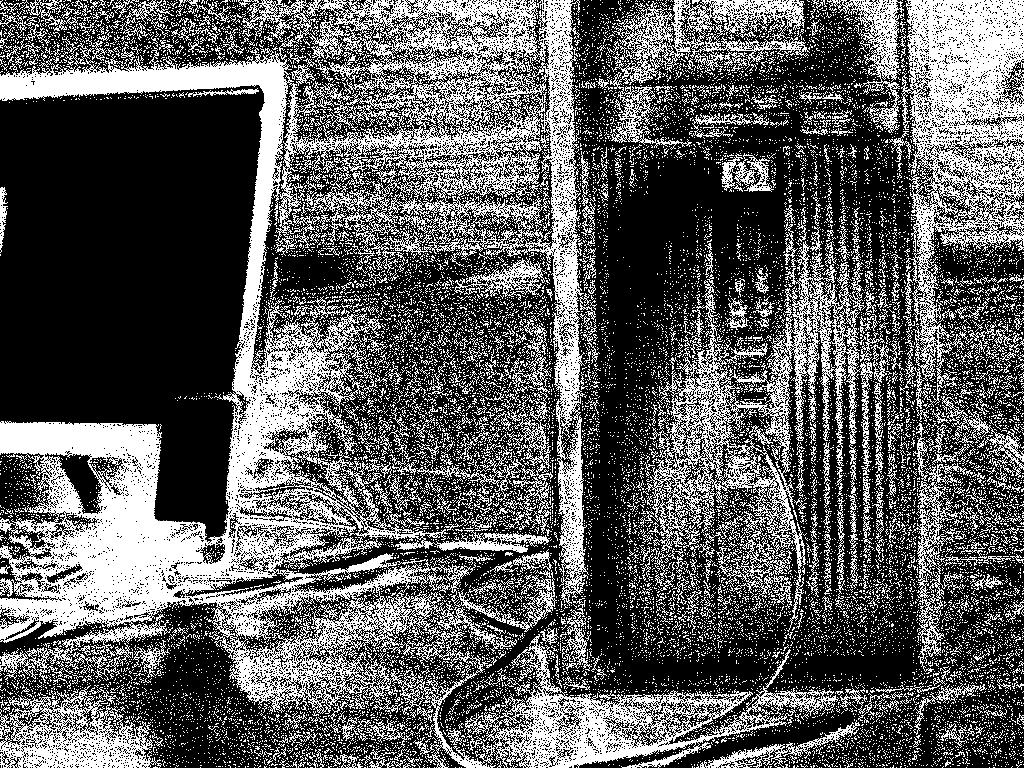
\includegraphics[width=0.3\linewidth]{Pictures/wolff/AOP.jpg}
	}
	\subfigure[Degree of Polarization $\rho$]{\label{fig:twoc}
	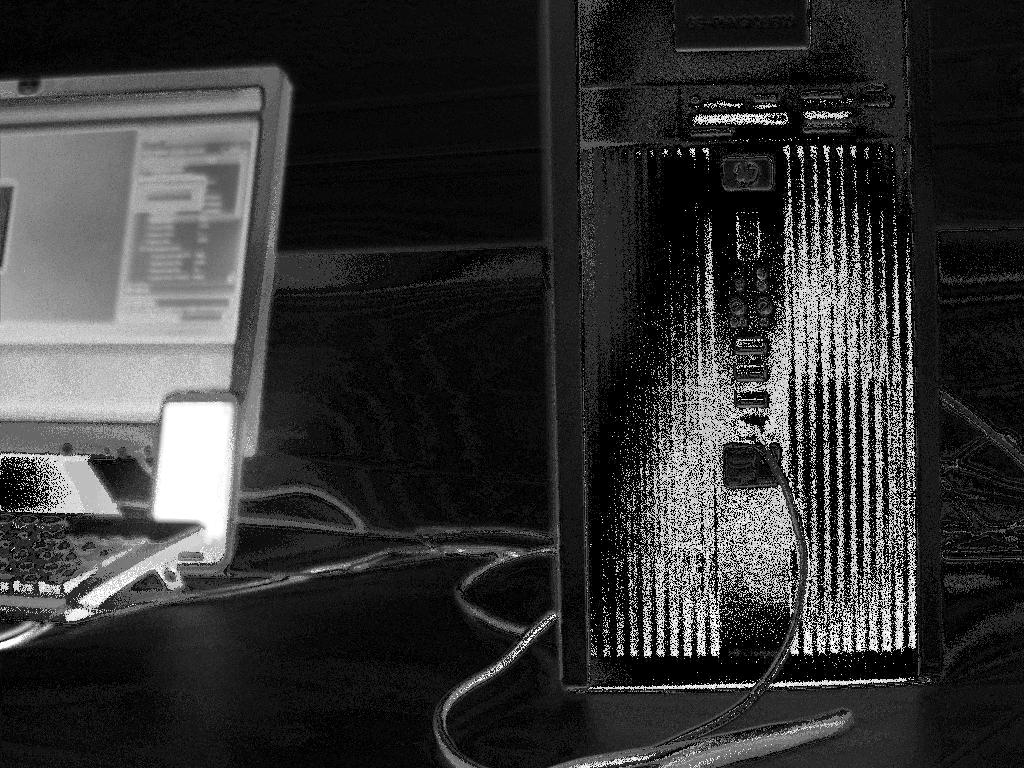
\includegraphics[width=0.3\linewidth]{Pictures/wolff/DOP.jpg}
	}
	\caption{Parameters of polarization}
	\label{fig:two}
\end{figure}

This part shows a color image that represents the three parameters, so we should wait a bit now.

\subsection{Least Mean Square method}
In this part, firstly we snap and store $N = 9$ images of one scene with $N$ consecutive orientations of polarizer. This images are shown in the Figure \ref{fig:three}.

\begin{figure}[H]
	\centering
	\subfigure[0\textdegree]{\label{fig:threea}
	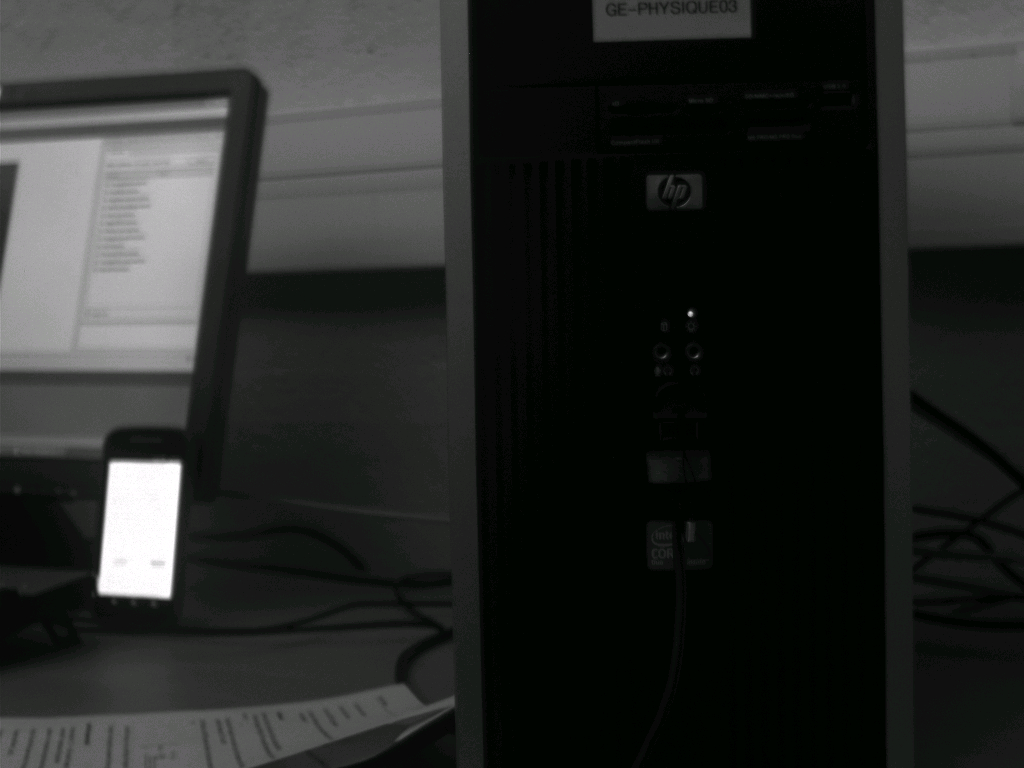
\includegraphics[width=0.3\linewidth]{Pictures/Least_Mean/0.jpg}
	}
	\subfigure[20\textdegree]{\label{fig:threeb}
	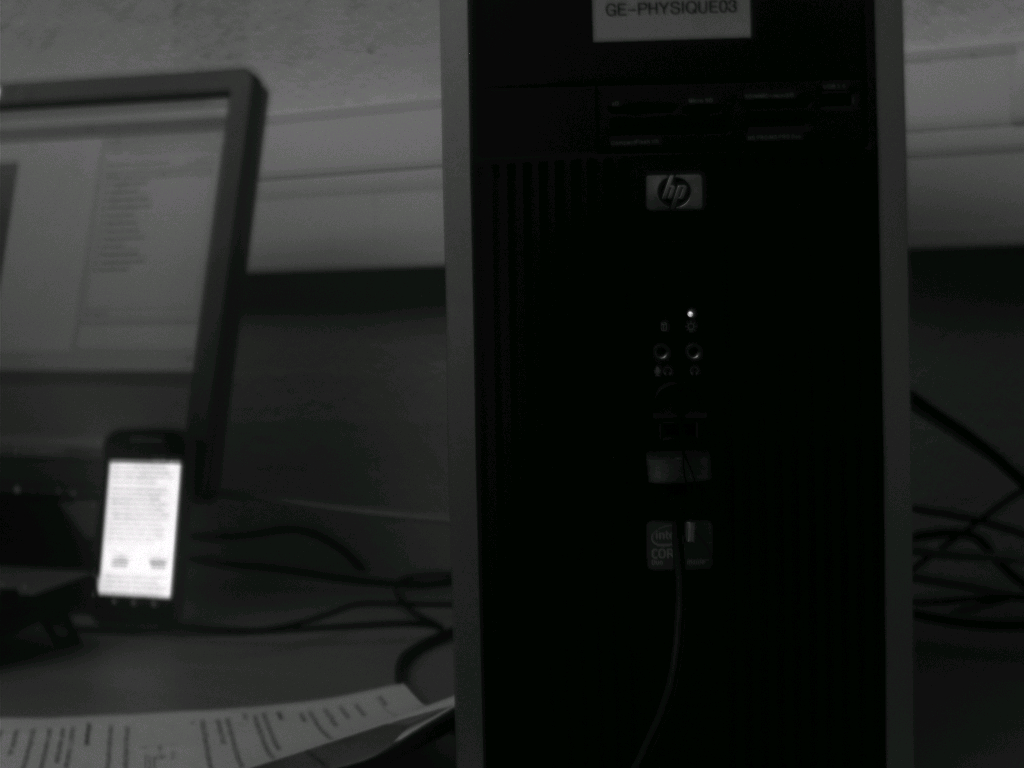
\includegraphics[width=0.3\linewidth]{Pictures/Least_Mean/20.jpg}
	}
	\subfigure[40\textdegree]{\label{fig:threec}
	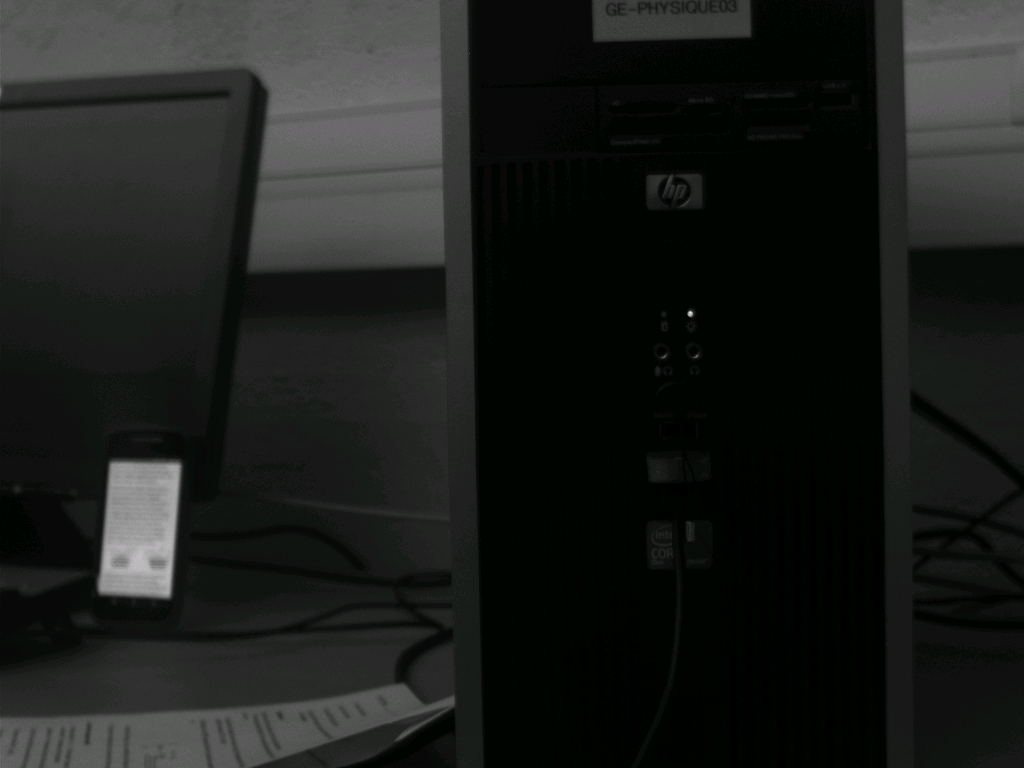
\includegraphics[width=0.3\linewidth]{Pictures/Least_Mean/40.jpg}
	}
	\subfigure[60\textdegree]{\label{fig:threed}
	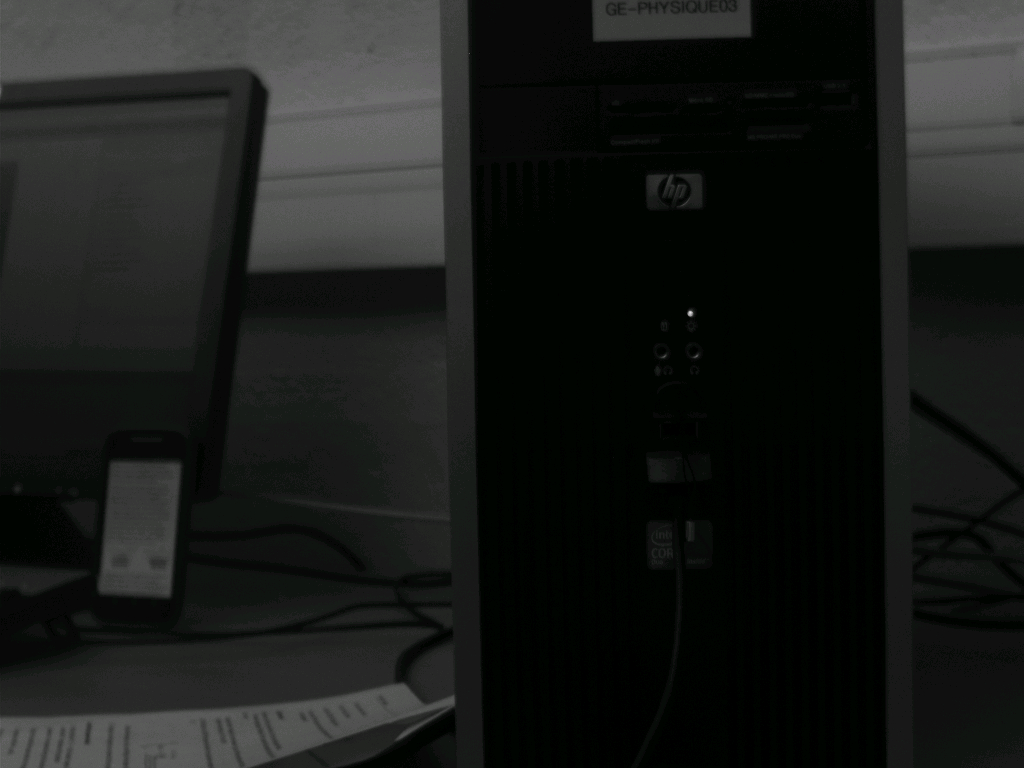
\includegraphics[width=0.3\linewidth]{Pictures/Least_Mean/60.jpg}
	}
	\subfigure[80\textdegree]{\label{fig:threee}
	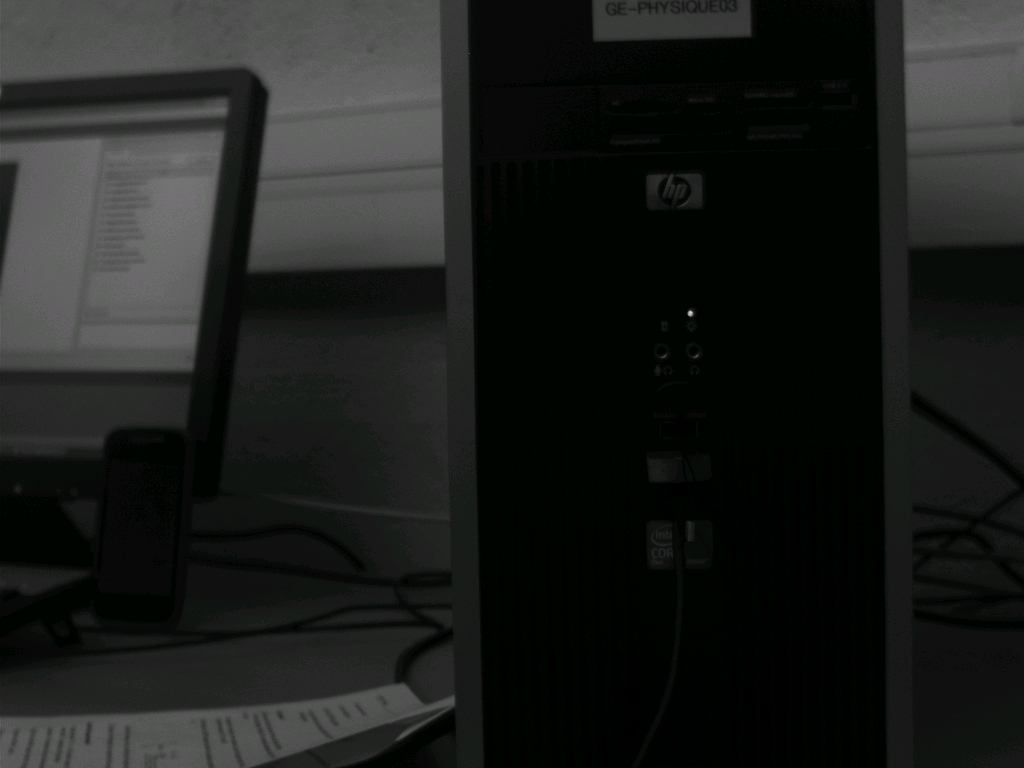
\includegraphics[width=0.3\linewidth]{Pictures/Least_Mean/80.jpg}
	}
	\subfigure[100\textdegree]{\label{fig:threef}
	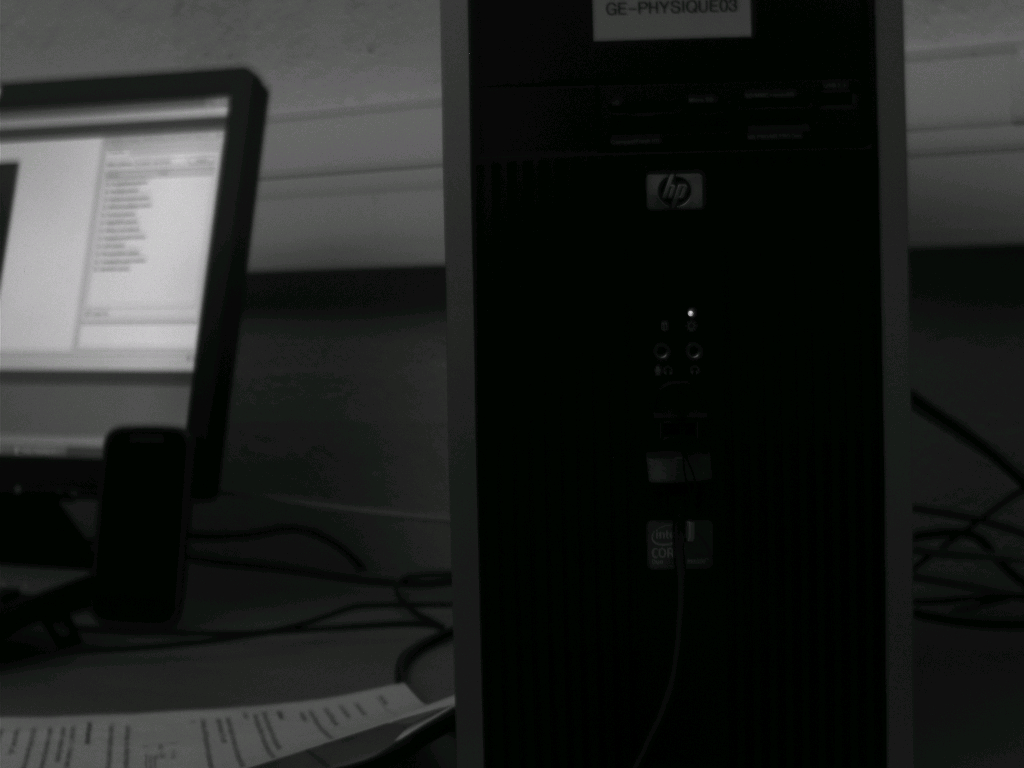
\includegraphics[width=0.3\linewidth]{Pictures/Least_Mean/100.jpg}
	}
	\subfigure[120\textdegree]{\label{fig:threeg}
	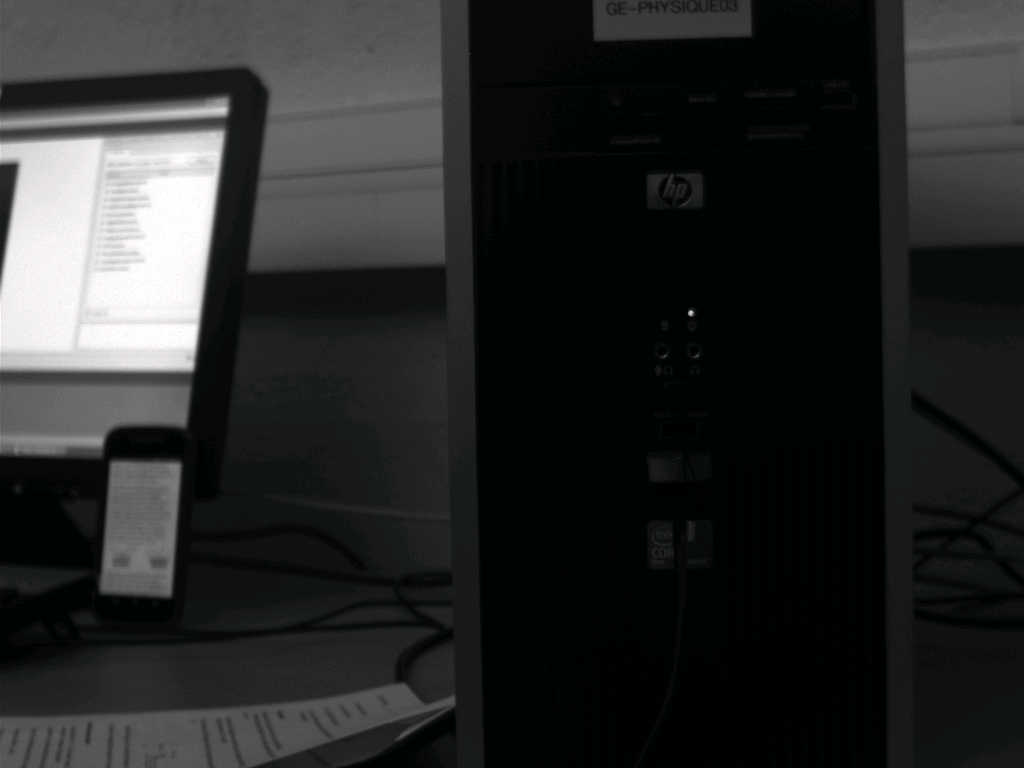
\includegraphics[width=0.3\linewidth]{Pictures/Least_Mean/120.jpg}
	}
	\subfigure[140\textdegree]{\label{fig:threeh}
	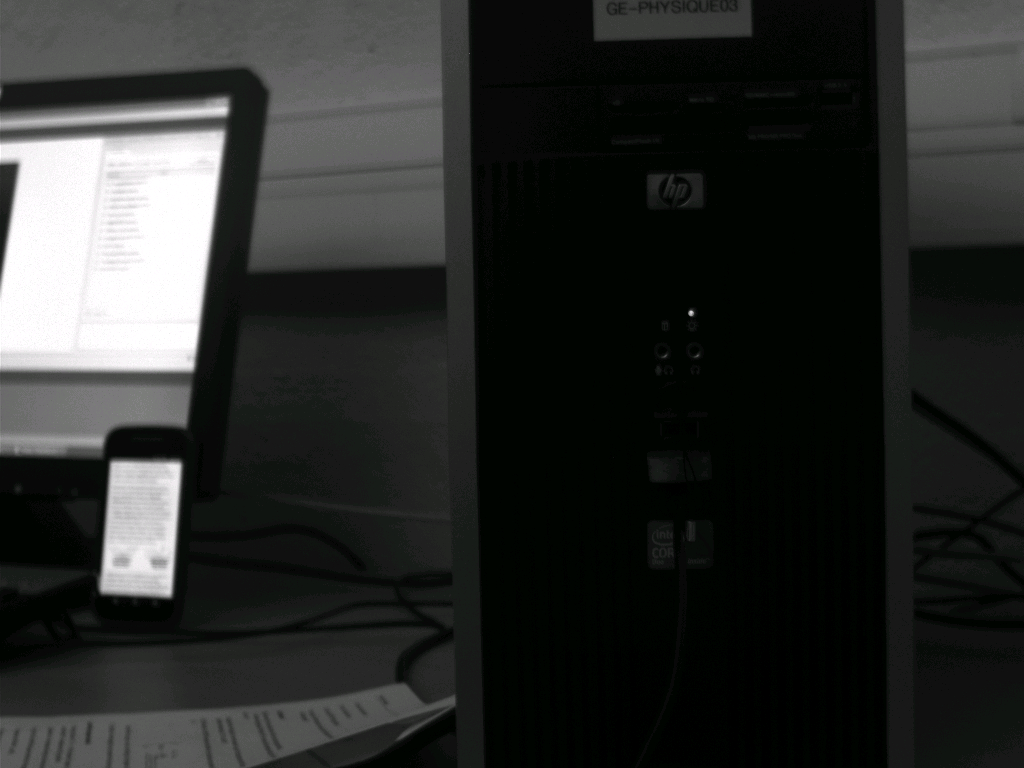
\includegraphics[width=0.3\linewidth]{Pictures/Least_Mean/140.jpg}
	}
	\subfigure[160\textdegree]{\label{fig:threei}
	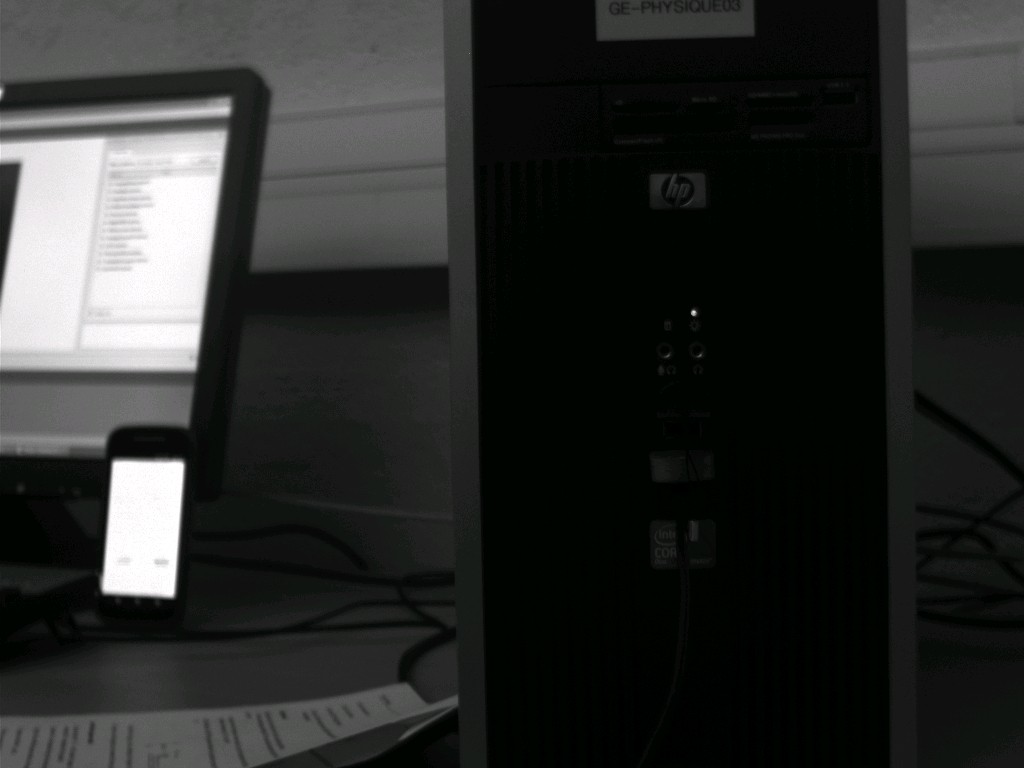
\includegraphics[width=0.3\linewidth]{Pictures/Least_Mean/160.jpg}
	}
	\caption{Images of a scene with various angles of polarizer (0\textdegree --160\textdegree)}
	\label{fig:three}
\end{figure}

After acquiring the $N$ pictures, we try to use Least Mean Square method to estimate $s_{0}, s_{1}, s_{2}$ based on the equation below. $M = rows\times columns$, for every pixel : $j = 1\dots M $, we have:
\begin{align*} 
	I^j_{1} &= 0.5(s^j_{0} + s^j_{1} cos2\alpha_{1} + s^j_{2} cos2\alpha_{1})\\
	I^j_{2} &= 0.5(s^j_{0} + s^j_{1} cos2\alpha_{2} + s^j_{2} cos2\alpha_{2})\\
	 &\dots \\
	I^j_{N} &= 0.5(s^j_{0} + s^j_{1} cos2\alpha_{N} + s^j_{2} cos2\alpha_{N})\\
\end{align*}
Where $I^j$ is the intensity value of one pixel, $\alpha$ corresponds to different angle of polarization. Such equations can be modelled as matrix form:
$$
Y = 0.5AX
$$
Here $X = [s_{0}, s_{1}, s_{2}]^T$. As we know, in this case, $A$ is a $9\times3$ matrix, whose rank is no bigger than 3. $Y$ has large possibility not belonging to the column space of $A$, so we have to use Least Mean Square method if we want to get a similar solution. Such a solution will be:
$$
X = (A^TA)^{-1}A^TY
$$

The images of $s_{0}, s_{1}, s_{2}$ is shown in Figure \ref{fig:four}.
\begin{figure}[H]
	\centering
	\subfigure[$s_{0}$]{\label{fig:foura}
	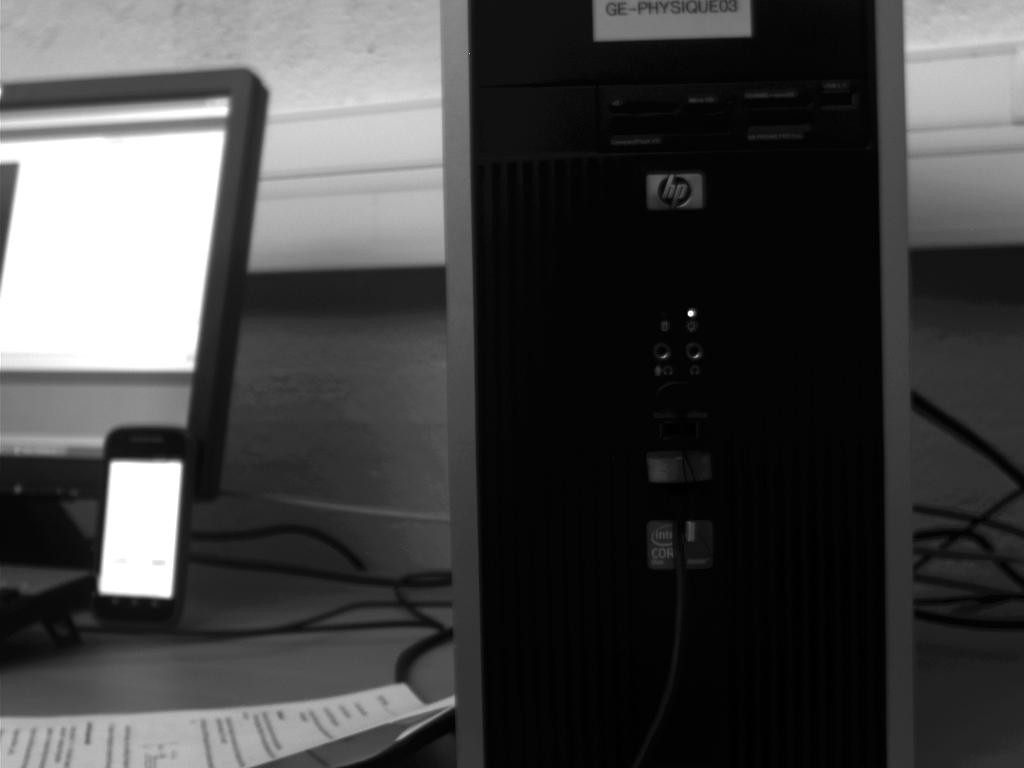
\includegraphics[width=0.3\linewidth]{Pictures/Least_Mean/S0.jpg}
	}
	\subfigure[$s_{1}$]{\label{fig:fourb}
	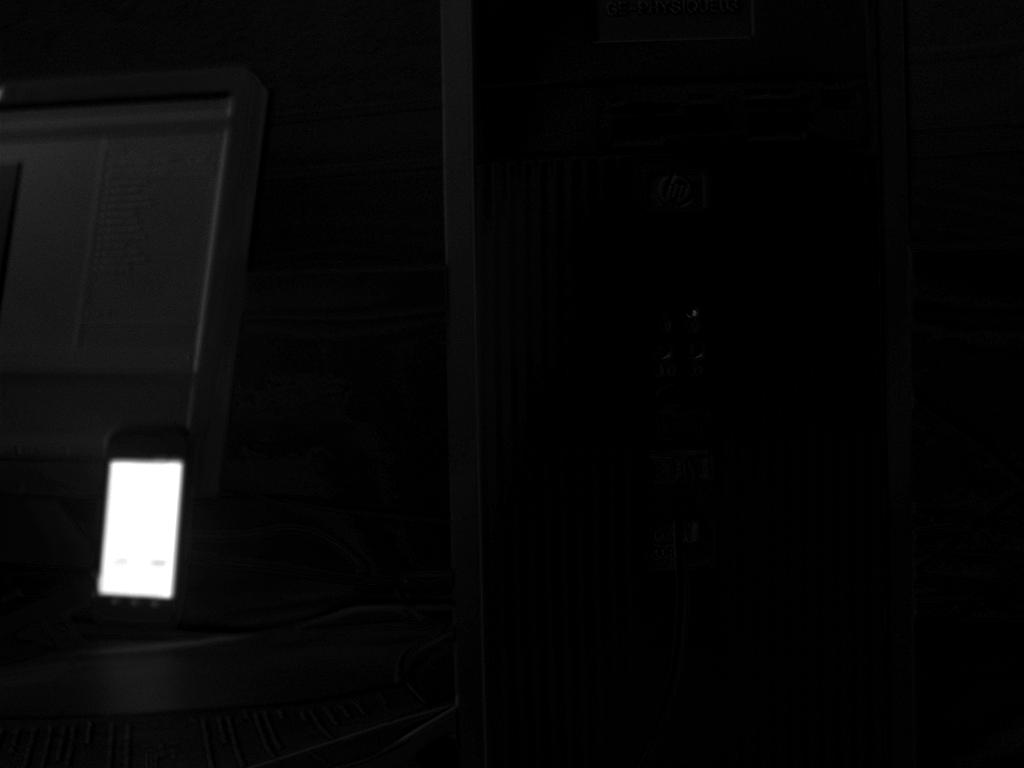
\includegraphics[width=0.3\linewidth]{Pictures/Least_Mean/S1.jpg}
	}
	\subfigure[$s_{2}$]{\label{fig:fourc}
	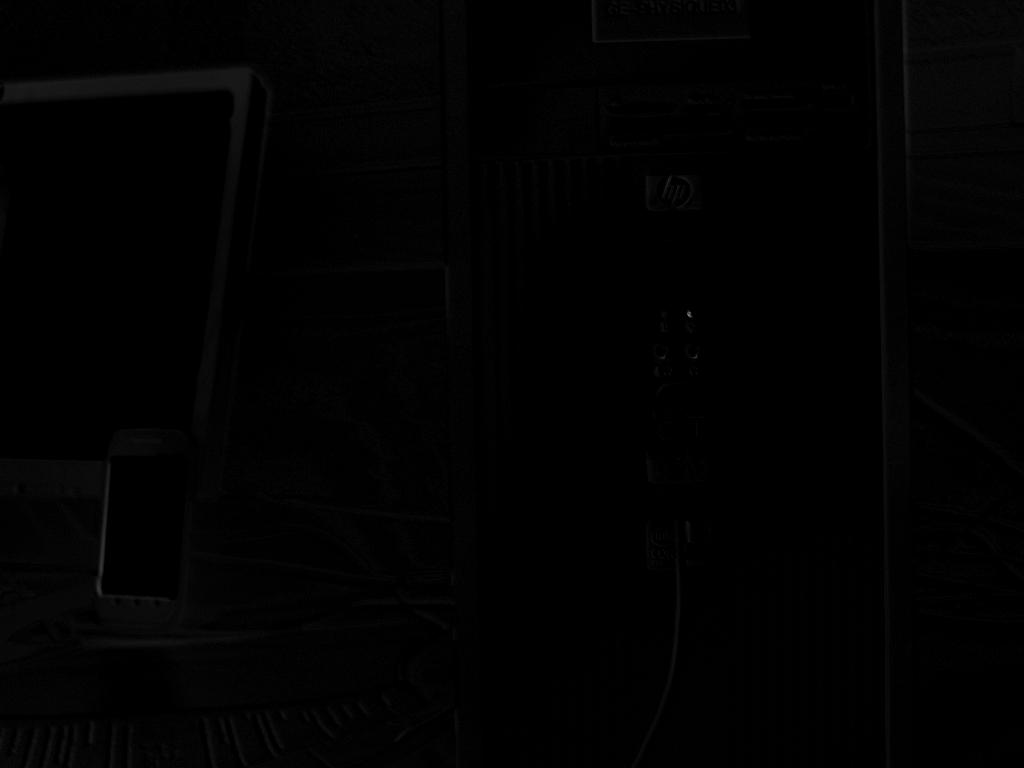
\includegraphics[width=0.3\linewidth]{Pictures/Least_Mean/S2.jpg}
	}
	\caption{Images of three parameters in Stokes Vector}
	\label{fig:four}
\end{figure}
Because we know the relationship below:\\
\\
\textbf{Toal light intenistiy} $I$
$$
I = s_{0}
$$
\textbf{Degree of polarization} $\rho$
$$
\rho = \frac{\sqrt{s_{1}^2  + s_{2}^2}}{s_{0}}
$$
\textbf{Angle of polarization} $\varphi$
$$
\varphi = 0.5\times atan(\frac{s_{2}}{s_{1}})
$$
Corresponding images are shown in Figure \ref{fig:five}
\begin{figure}[H]
	\centering
	\subfigure[$I$]{\label{fig:fivea}
	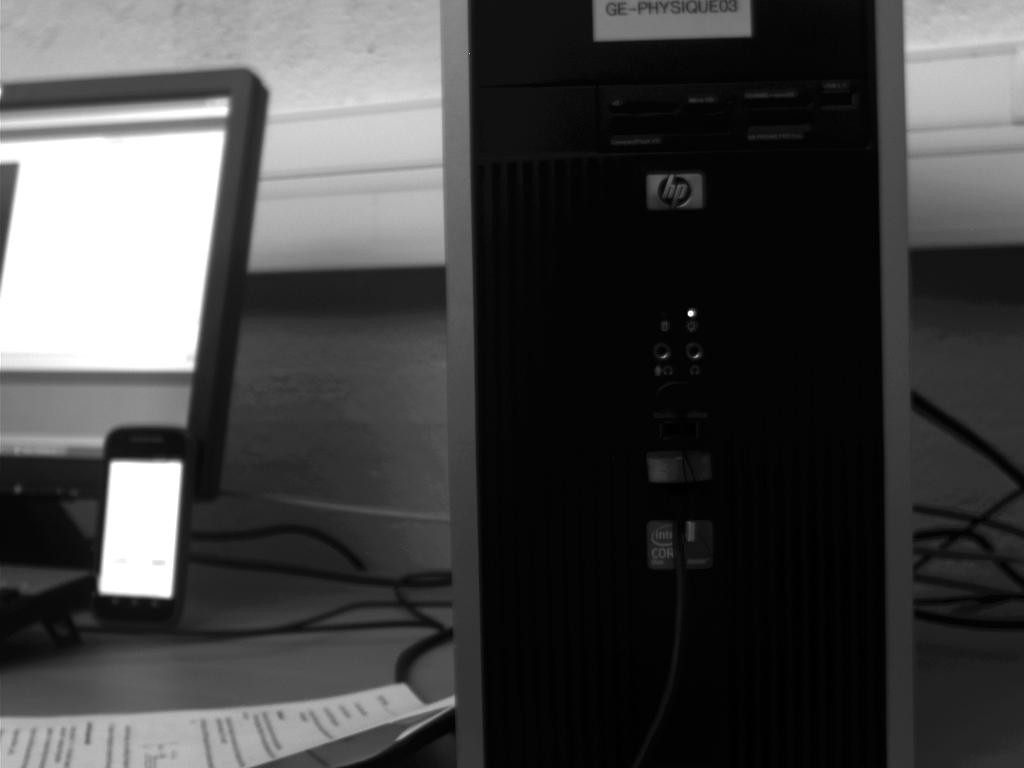
\includegraphics[width=0.3\linewidth]{Pictures/Least_Mean/I_Least.jpg}
	}
	\subfigure[$\rho$]{\label{fig:fiveb}
	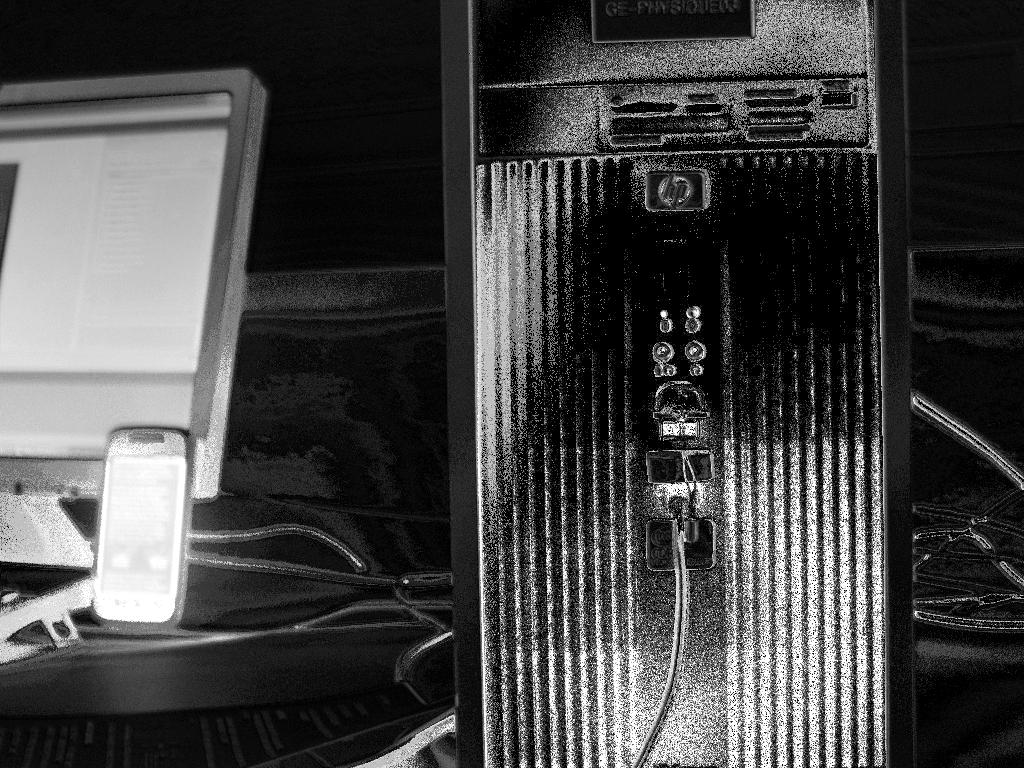
\includegraphics[width=0.3\linewidth]{Pictures/Least_Mean/DOP_Least.jpg}
	}
	\subfigure[$\varphi$]{\label{fig:fivec}
	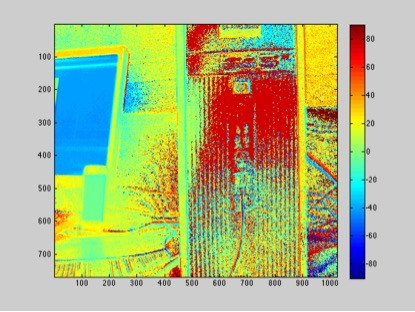
\includegraphics[width=0.3\linewidth]{Pictures/Least_Mean/Phi_Least.jpg}
	}
	\caption{$I, \rho, \varphi$}
	\label{fig:five}
\end{figure}

Draw sinusoidal relationship part

\section{Contrast polarization measurement}
In this section we use two polarizer, an electronic rotator and a light source to explore the properties of objects and light reflections.\\

\subsection{Polarizers and a rotator}
First, we experimented with different setting of polarizers and observed the effect of the angle between polarizers on the image( Figure \ref{fig:six}).\\

\begin{figure}[H]
	\centering
	\subfigure[0\textdegree]{\label{fig:2pol0}
	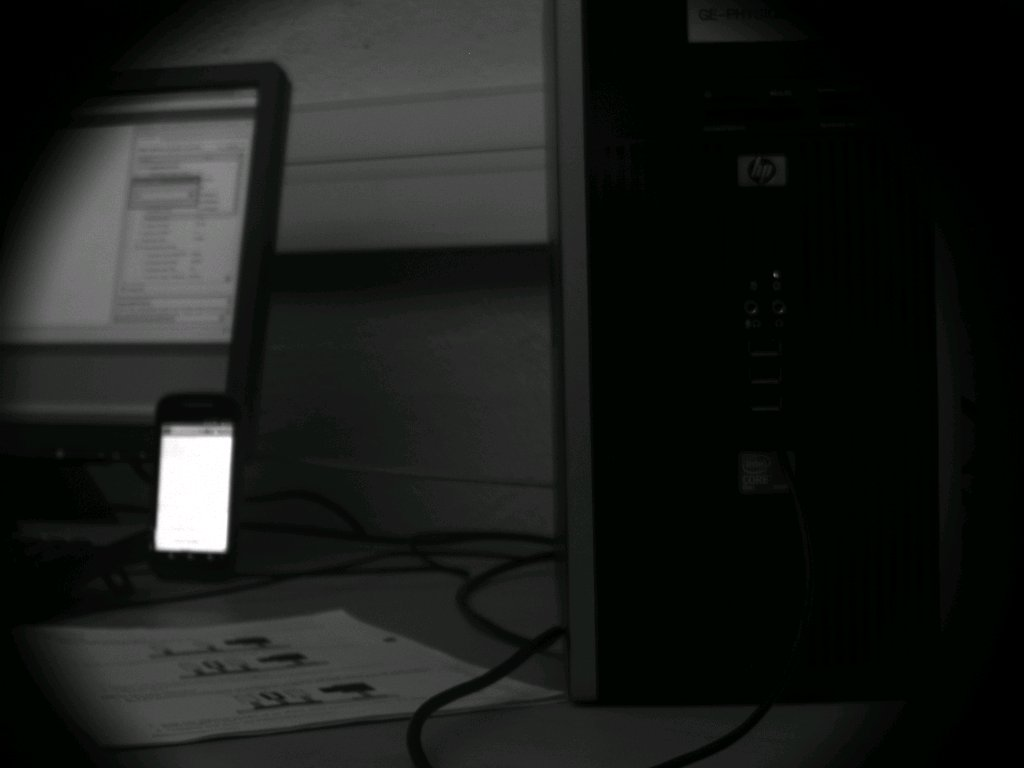
\includegraphics[width=0.3\linewidth]{Pictures/contrast/00.jpg}
	}
	\subfigure[45\textdegree]{\label{fig:2pol45}
	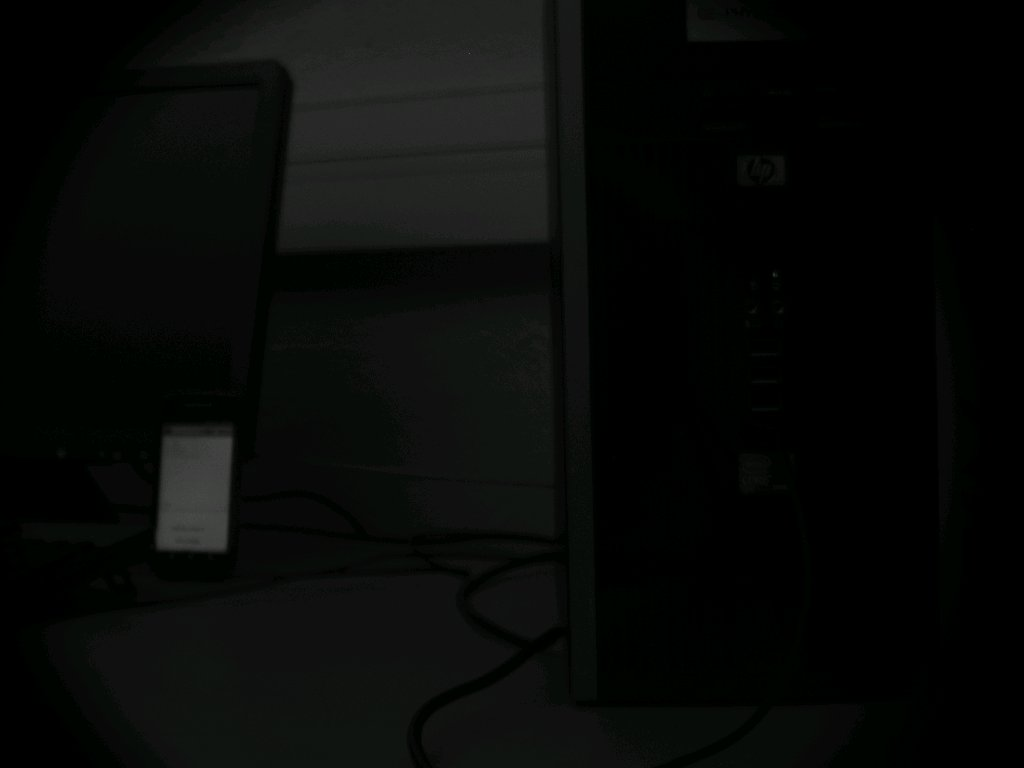
\includegraphics[width=0.3\linewidth]{Pictures/contrast/0-45.jpg}
	}
	\subfigure[90\textdegree]{\label{fig:2pol90}
	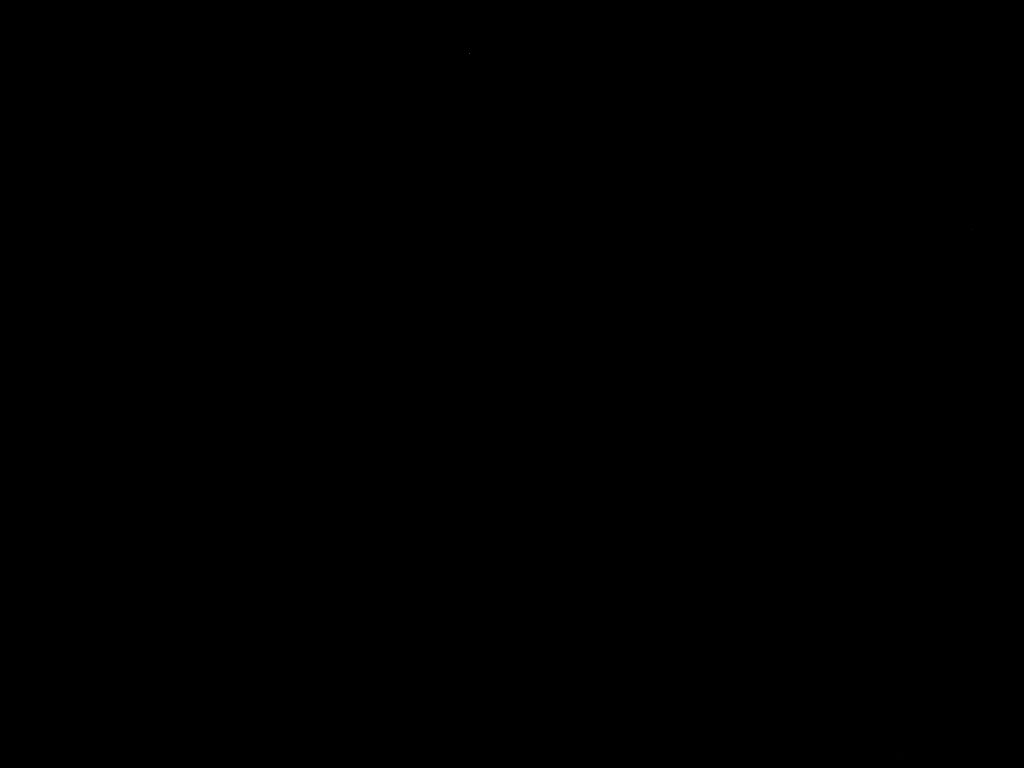
\includegraphics[width=0.3\linewidth]{Pictures/contrast/90-0.jpg}
	}
	\caption{Different settings of two polarizers}
	\label{fig:six}
\end{figure}
When we set up the two polarizers oriented to $0\deg$ we saw that the intensity of the light decreases with adding each polarizer. 
After the first polarizer, the light is dimmed a little bit. According to Malus' law:
$I=I_ocos^2(θ)$\\
Where $I_0$ is the initial intensity and $\Theta$ is the angle of polarization.\\
That means that when the light is not polarized, only a half of the light will be transmitted as the cosine term will average to $\frac{1}{2}$\\
After the first polarizer, the light is linearly polarised, and again, according to Malus' Law it is diminished depending in the angle $\Theta$.\\
From there we can conclude, that if the angle of polarisation $\Theta$ is $0\deg$, the intensity remains the same as after the first polarizer: 1 / 2 of initial intensity. \\
After that the switchable polarization rotator is inserted between two polarizers.
This rotator has only two states: rotate light by $90\deg$ or $0\deg$. 
So when the polarizers are set to $0\deg$ each and the rotator is on, the light is rotated by $90\deg$, making it perpendicular to the second polarizer. 
That, as we know results in total extinguishing of any light passing. 
However when the rotator is off, there is almost no difference.\\
\begin{figure}[H]
	\centering
	\subfigure[0\textdegree]{\label{fig:rotatorzero}
	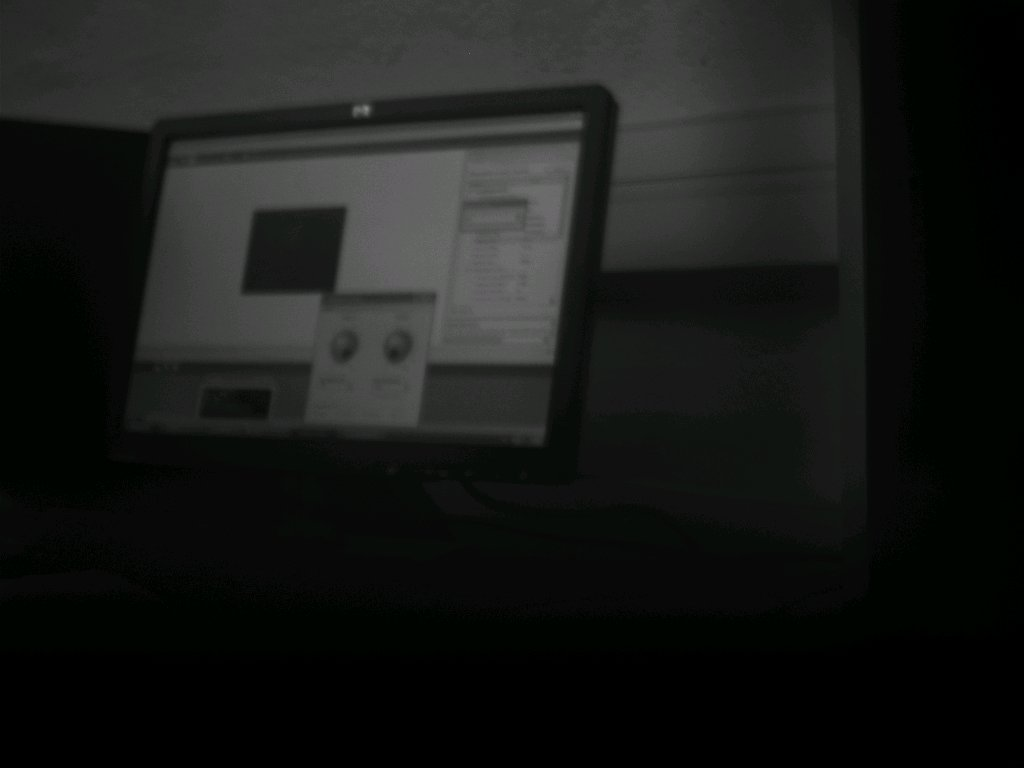
\includegraphics[width=0.3\linewidth]{Pictures/retarder/0.jpg}
	}
	\subfigure[90\textdegree]{\label{fig:rotatorninety}
	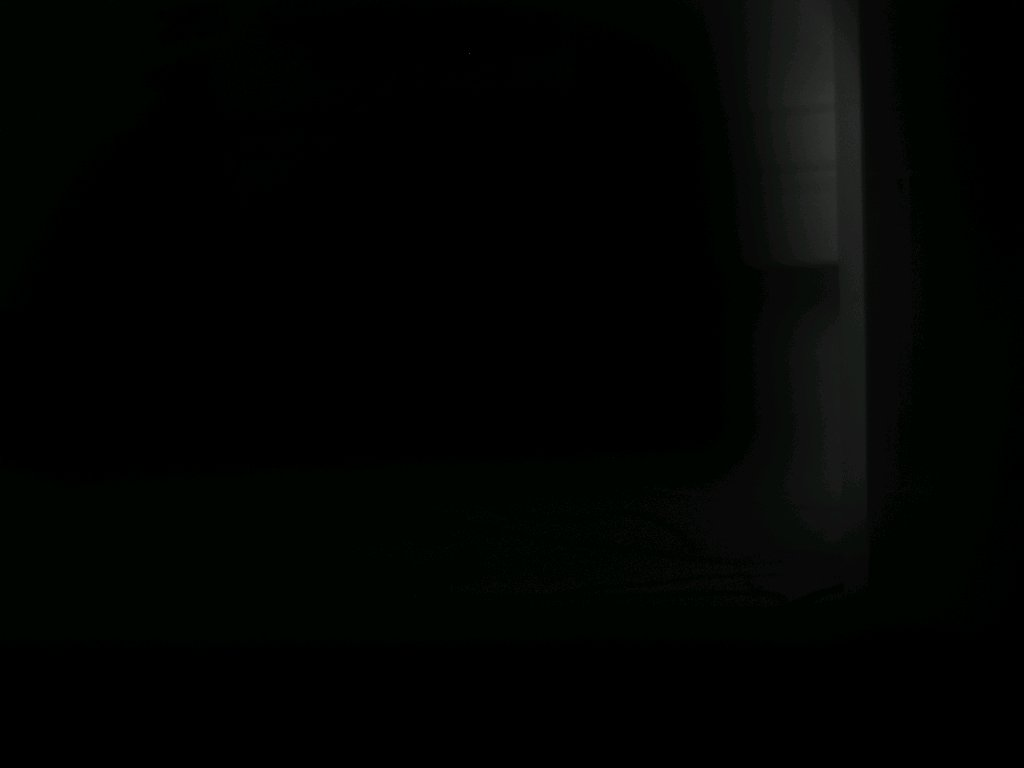
\includegraphics[width=0.3\linewidth]{Pictures/retarder/90.jpg}
	}
	\caption{polarizer with a rotator(off in the first image, and on in the second)}
	\label{fig:seven}
\end{figure}

\subsection{Diffused and specular reflection}
In this section we experiment with diffused and specular reflections, and how the polarizer affects that kind of light.\\
Specular reflection can be seen when light is reflected from smooth surfaces and the reflected light becomes polarised.
Diffused reflection is caused when light falls onto a rough surface. 
This reflected light is not polarised but diffused in all directions.\\
To test that, we introduced a polarised light source into the system, before the rotator. \\
We observe that the glare of light is mostly removed from the shiny surface, while the intensity is only dimmed for the diffused reflection as expected.\\

\begin{figure}[H]
	\centering
	\subfigure[0\textdegree]{\label{fig:rotatorzero}
	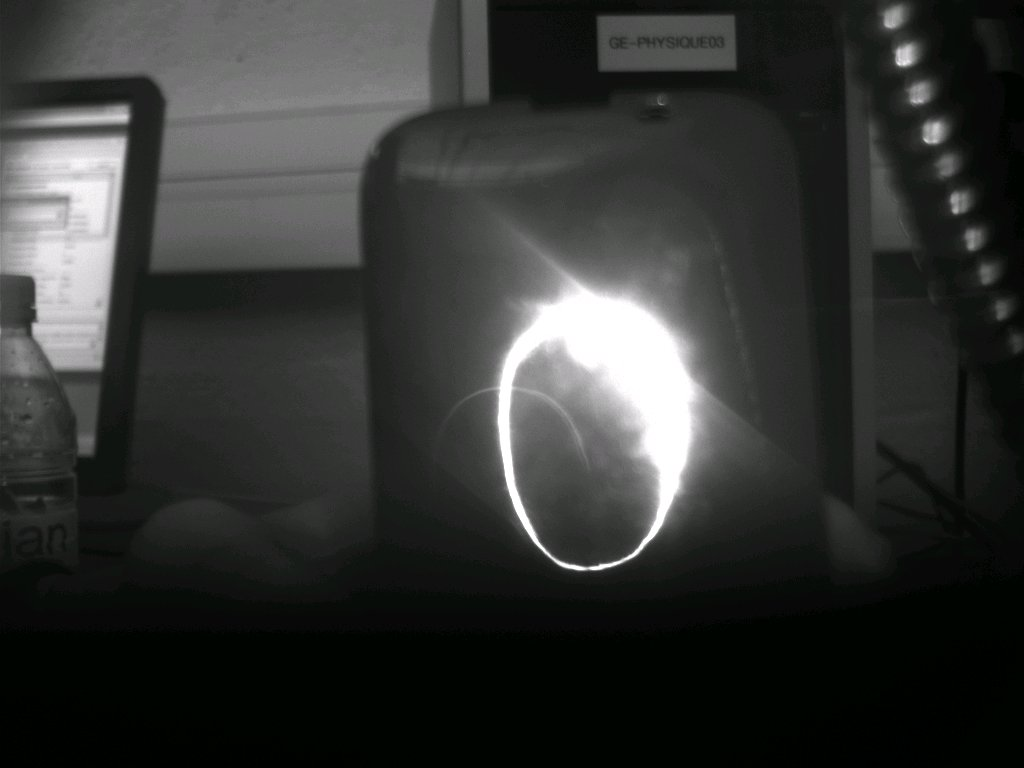
\includegraphics[width=0.3\linewidth]{Pictures/reflect/0.jpg}
	}
	\subfigure[0\textdegree]{\label{fig:rotatorninety}
	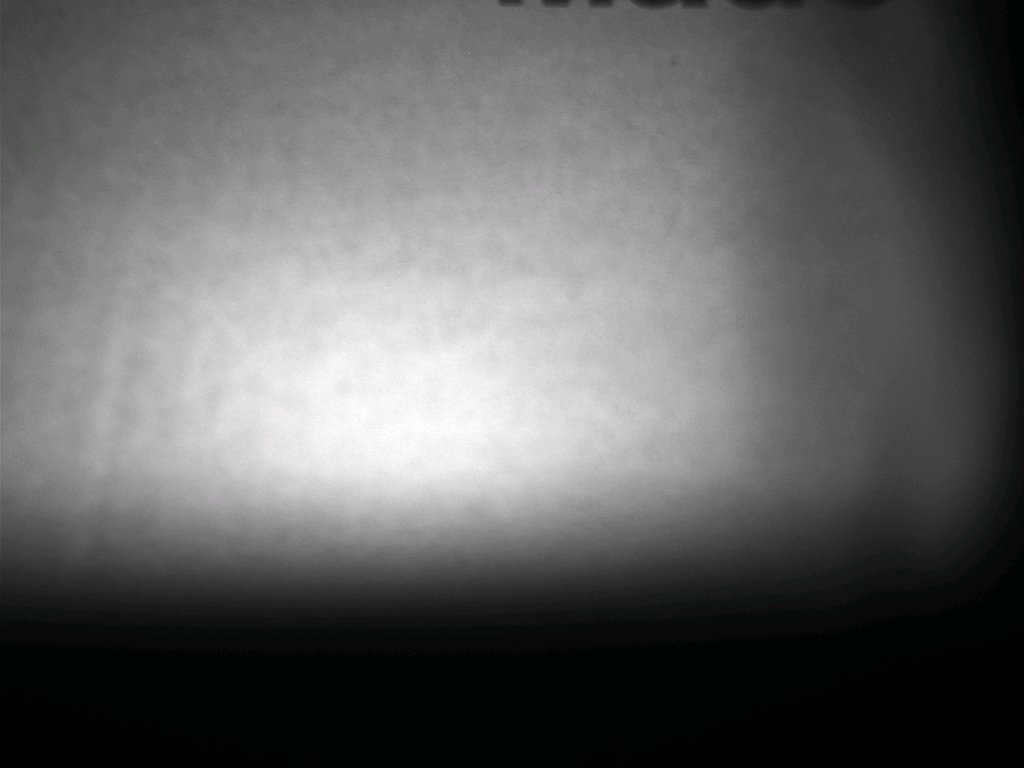
\includegraphics[width=0.3\linewidth]{Pictures/reflect/d0.jpg}
	}
	\caption{Specular and diffused reflection with polarizer, rotator:off}
	\label{fig:eight}
\end{figure}

\begin{figure}[H]
	\centering
	\subfigure[90\textdegree]{\label{fig:rotatorzero}
	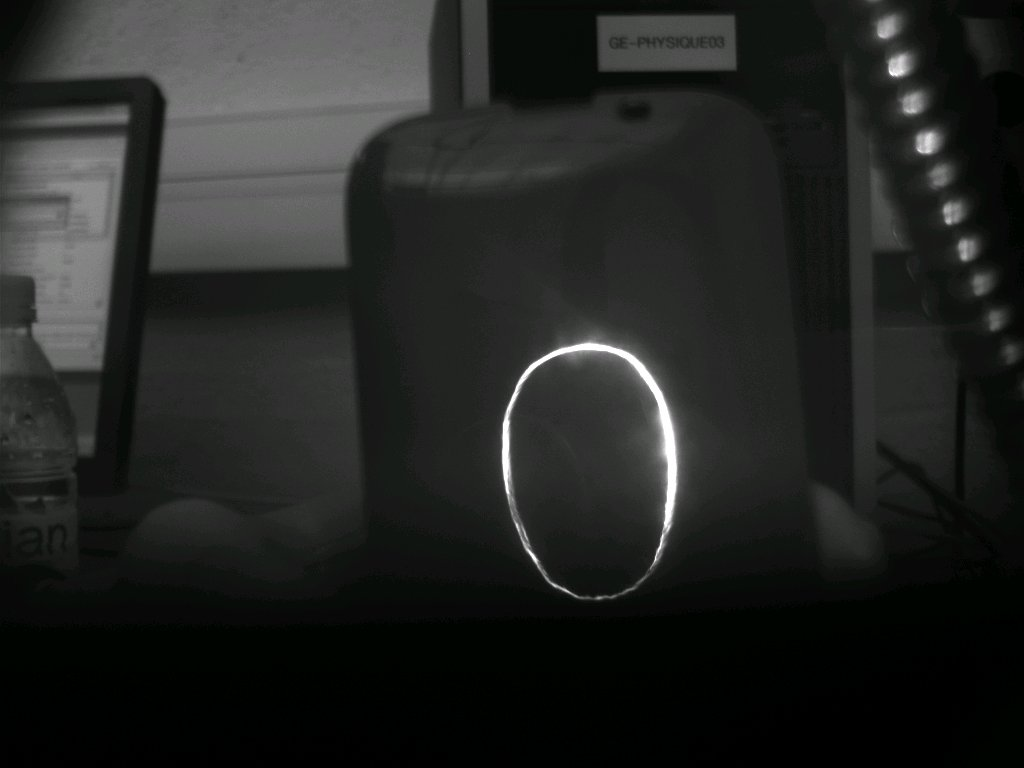
\includegraphics[width=0.3\linewidth]{Pictures/reflect/90.jpg}
	}
	\subfigure[90\textdegree]{\label{fig:rotatorninety}
	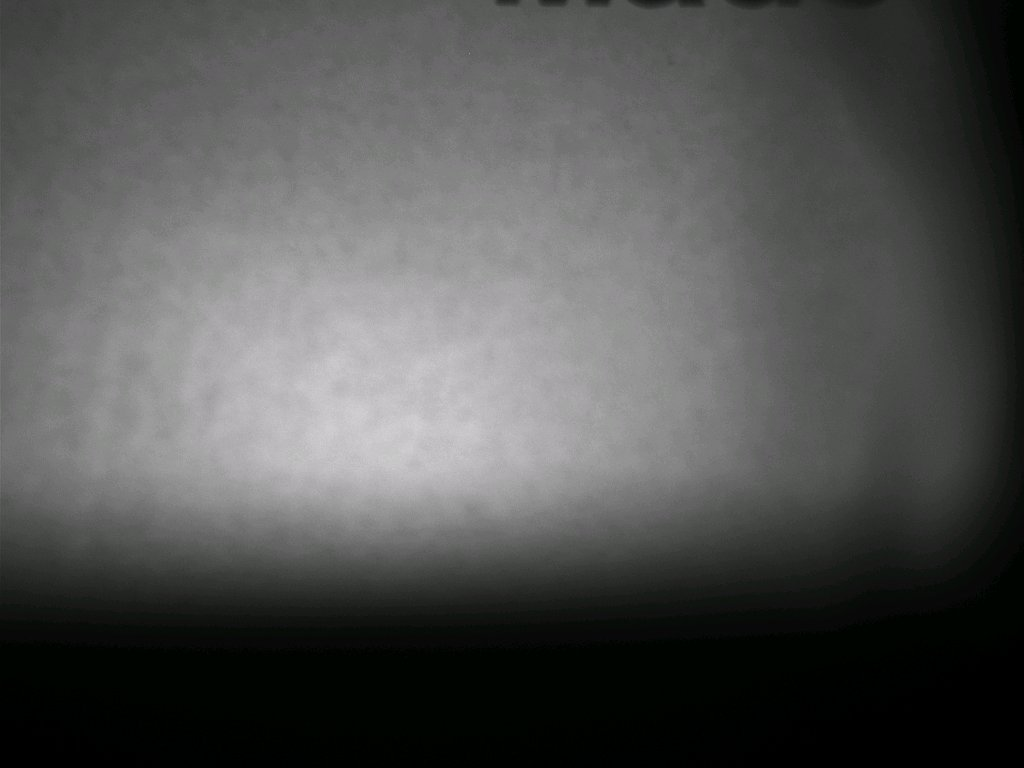
\includegraphics[width=0.3\linewidth]{Pictures/reflect/d90.jpg}
	}
	\caption{Specular and diffused reflection with polarizer, rotator:on}
	\label{fig:nine}
\end{figure}
From the obtained images we can compute the polarization contrast ratio:\\
\begin{center}
$PCR = \frac{I_{contrast}}{I_{total}}$,
where\\

$I_{total} = I_{\parallel} + I_{\perp}$ 
and 
$I_{contrast} = I_{\parallel} - I_{\perp}$
\end{center}
The contrast ratio describes the properties of the polarizer itself, as it is the ratio of transmitted light when the polarizers are parallel to the transmission when they are crossed, as seen from the formulas above.\\
To compute the contrast ratio, we used the images in Figures $\ref{fig:eight}$ $\ref{fig:nine}$ so that $I_{\parallel}$ and $I_{\parallel}$ are the images with $0\deg$ and $90\deg$ angles respectively.\\
\begin{figure}[H]
	\centering
	\subfigure[Total $I$]{\label{fig:a}
	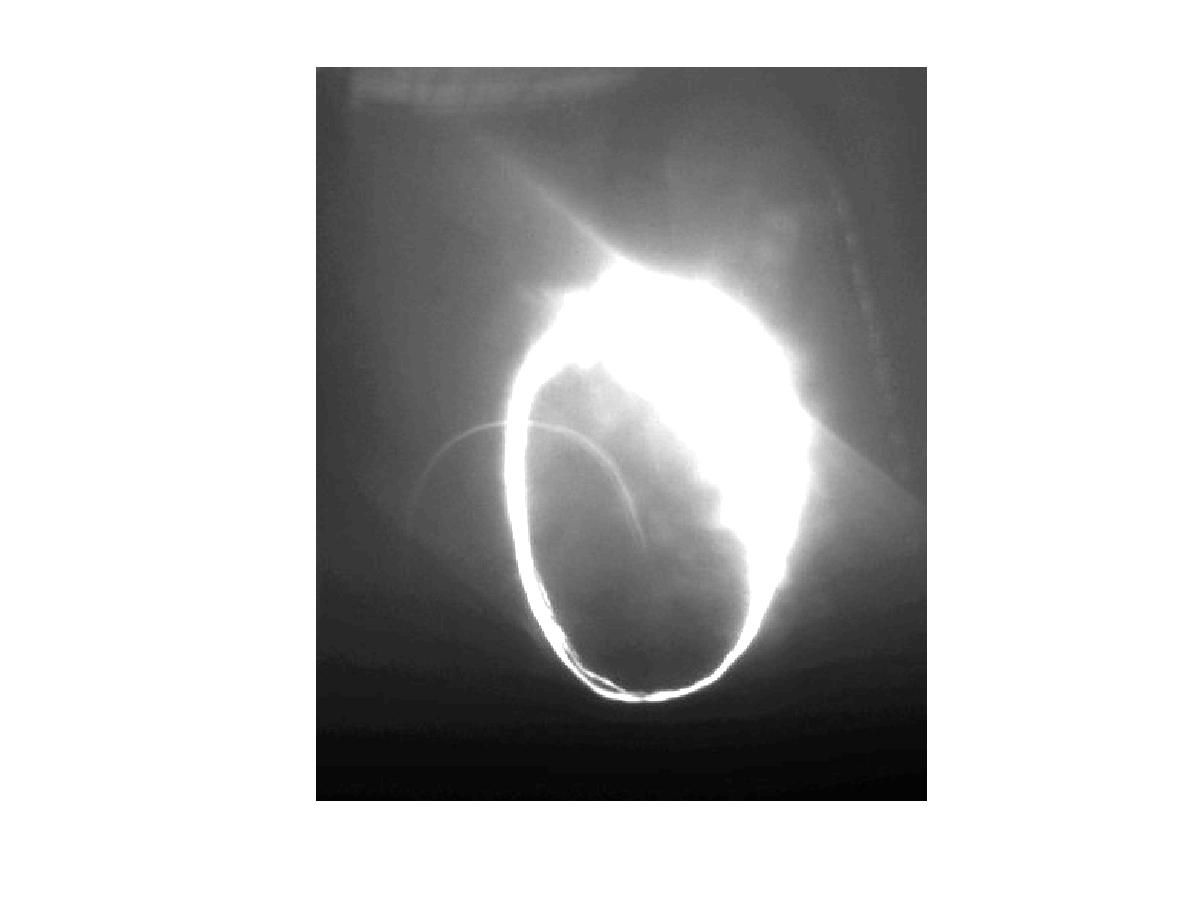
\includegraphics[width=0.3\linewidth]{Pictures/reflect/stotal.jpg}
	}
	\subfigure[Contrast]{\label{fig:b}
	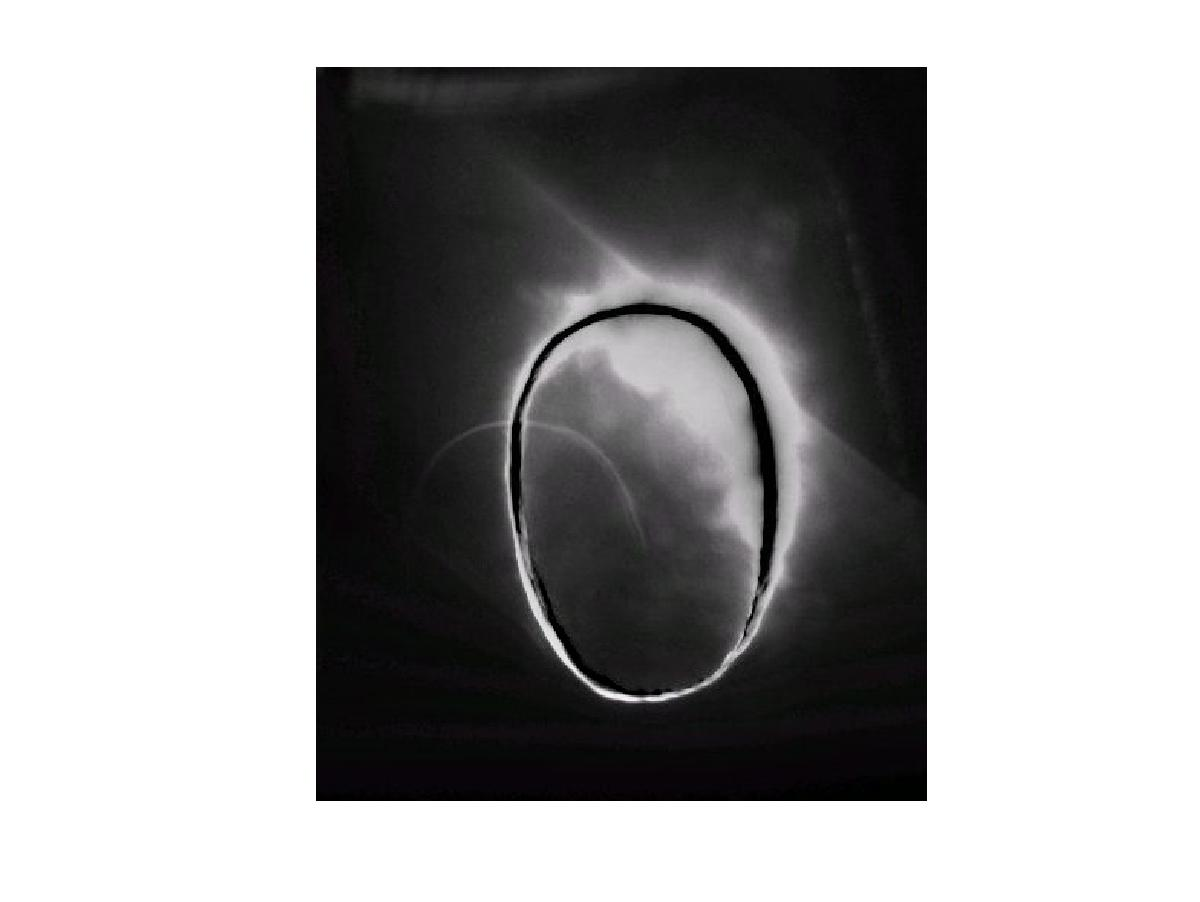
\includegraphics[width=0.3\linewidth]{Pictures/reflect/scontrast.jpg}
	}
	\subfigure[Contrast ratio]{\label{fig:c}
	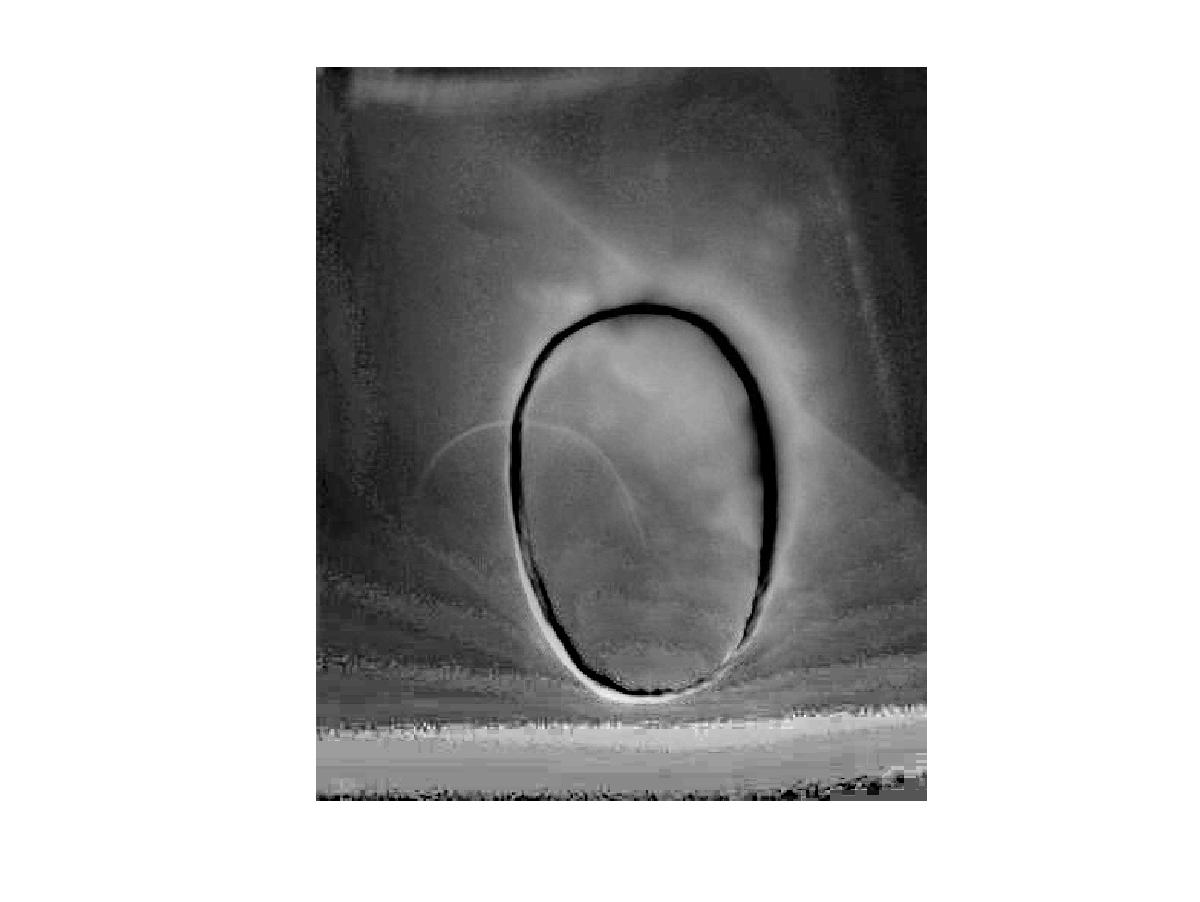
\includegraphics[width=0.3\linewidth]{Pictures/reflect/sratio.jpg}
	}
	\caption{Total and contrast intensities and their ratio for specular reflection}
	\label{fig:ten}
\end{figure}
In the images we can clearly see the filtered glare of light when the polarizer and the light were crossed in the contrast image.\\
After doing the same computations for diffused reflection the following results were obtained:
\begin{figure}[H]
	\centering
	\subfigure[Total $I$]{\label{fig:a}
	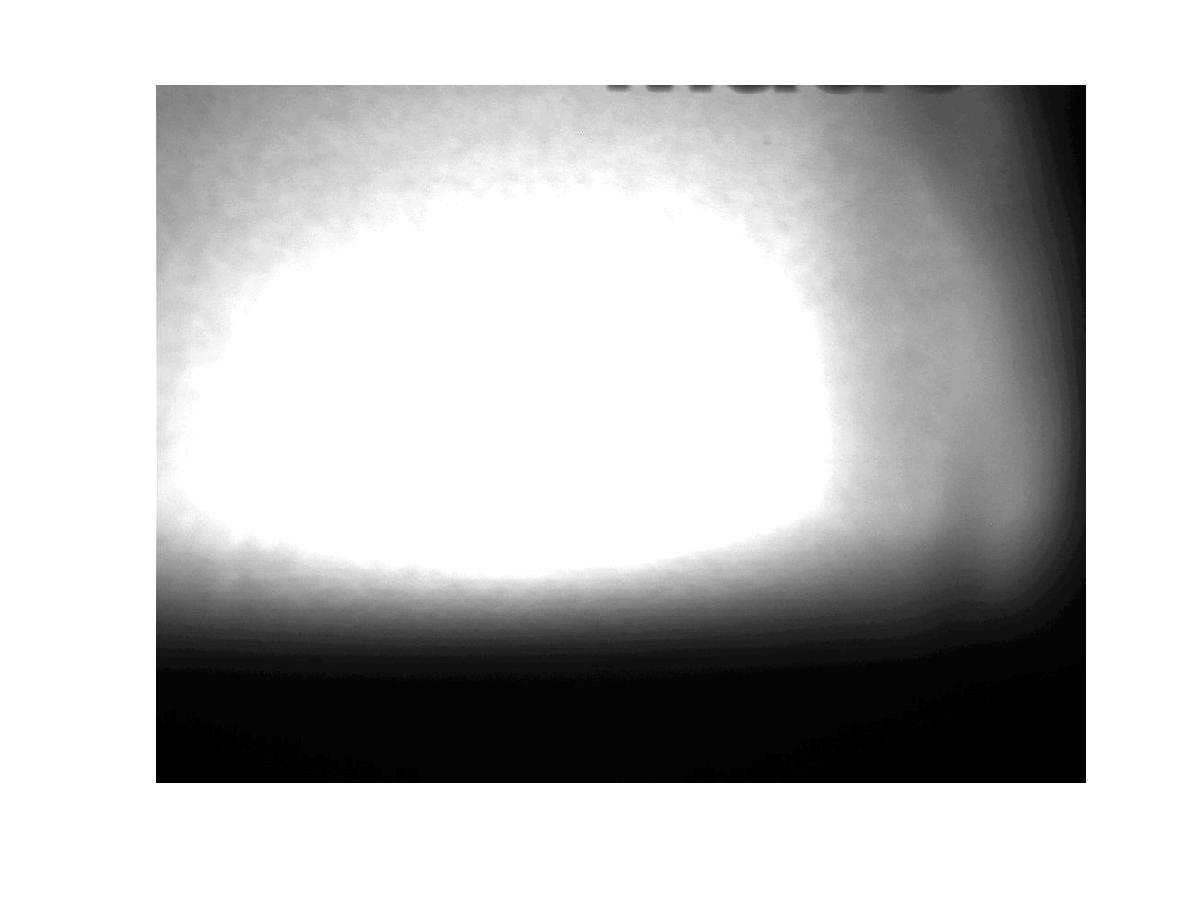
\includegraphics[width=0.3\linewidth]{Pictures/reflect/dtotal.jpg}
	}
	\subfigure[Contrast]{\label{fig:b}
	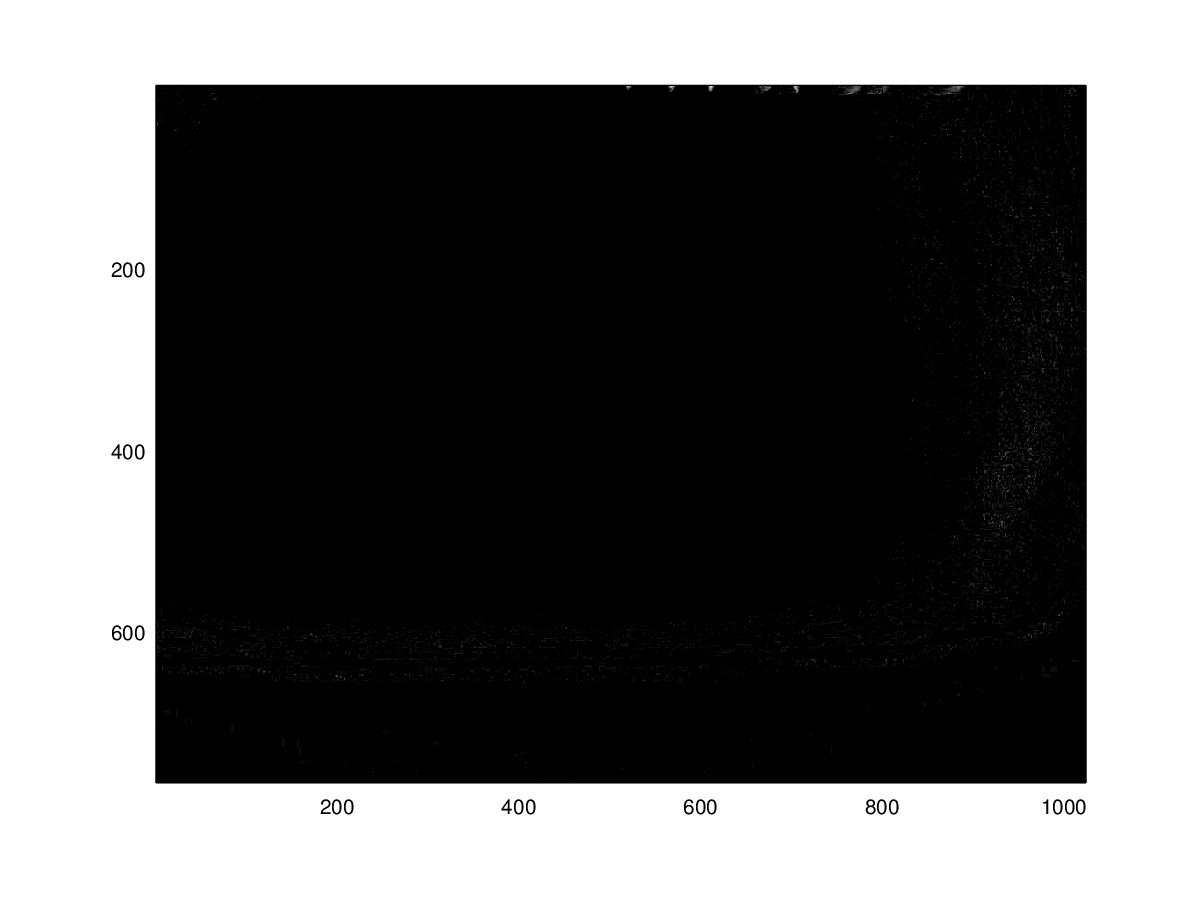
\includegraphics[width=0.3\linewidth]{Pictures/reflect/dcontrast.jpg}
	}
	\subfigure[Contrast ratio]{\label{fig:c}
	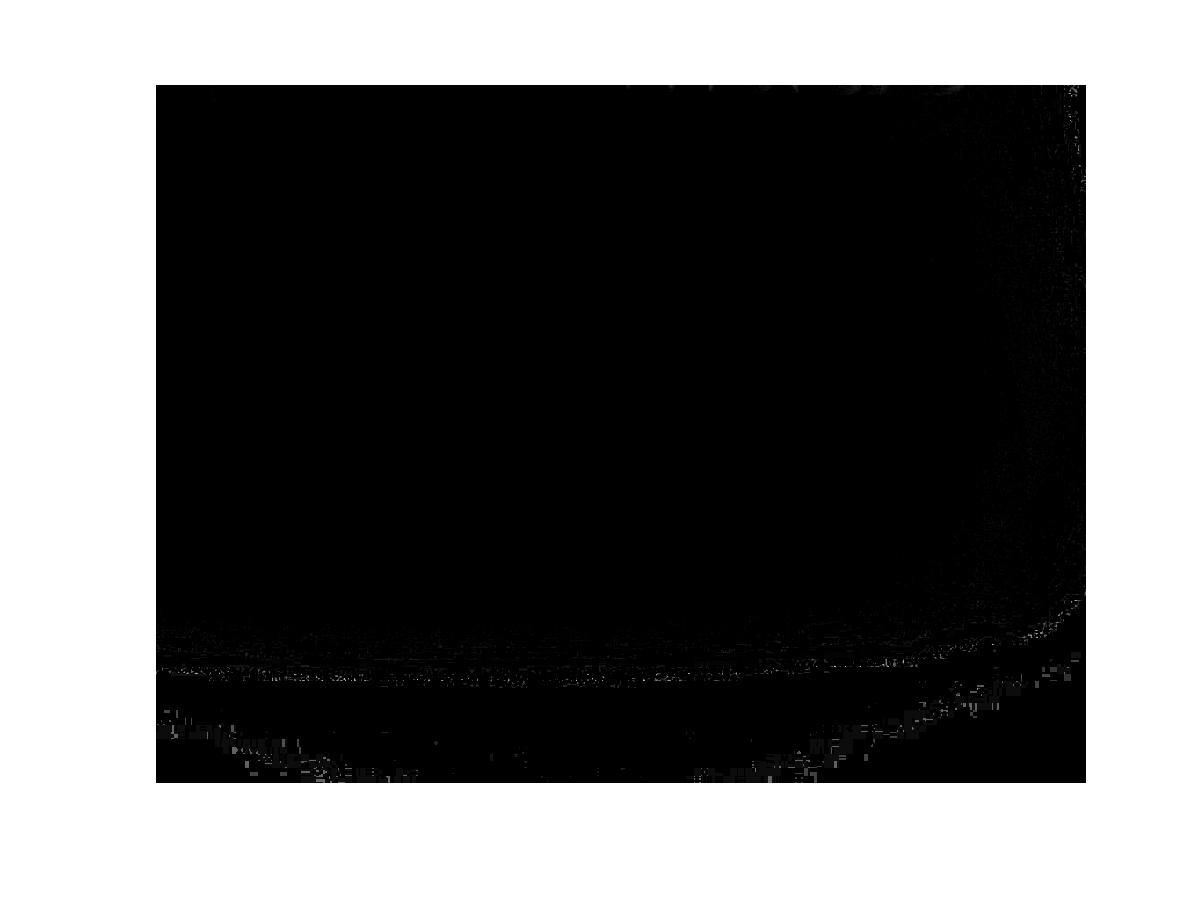
\includegraphics[width=0.3\linewidth]{Pictures/reflect/dratio.jpg}
	}
	\caption{Total and contrast intensities and their ratio for diffused reflection}
	\label{fig:eleven}
\end{figure}
These images are for diffused reflection, and as we know diffused reflection is only slightly affected by polarizers.
Hence, the difference between $0\deg$ and $90\deg$ angles of polarization is so small that it is almost invisible.\\
\section{Conclusion}
In this laboratory work we experimented with polarizers and their properties. 
After capturing the resulting imaging with a camera, we were able to measure the parameters of polarized light.
We also explored the properties of diffused and specular reflections and how they are affected by polarizers.

\section{References}

{[}1{]} -https://en.wikipedia.org/wiki/Polarizer\\
{[}2{]} -http://www.semrock.com/Data/Sites/1/semrockpdfs/whitepaper\_anewclassofpolarizationopticsforlasers.pdf

\end{document}